%!TEX root = manual.tex
%===============================================================================
\chapter{Distributed housekeeping program}\label{ch:Assignment5}

The two previous versions of the housekeeping program display the measured values on a debugger console. This means that the program must be run from the debugger, with the ST-LINK cable in place.

A more realistic solution uses a serial interface to send these values to a simulated ground station running on the host computer, as shown in figure~\ref{fig:architecture}). The aim is to simulate the radio link between the satellite and the ground station.

\section{Serial line connections.}\label{sc:serial}

This scheme makes use of the USB/UART interface cable provided to the students. The USB/ UART cable has a TTL connector that must be connected to the STM32f4 board pins that convey the serial line (UART) signals (figure~\ref{fig:cable}).

\begin{figure}[h]
            \centering{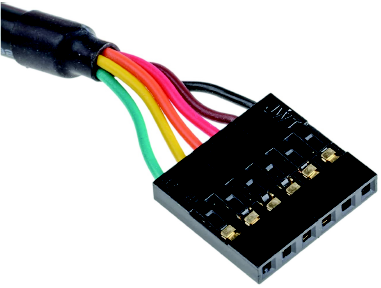
\includegraphics[width=0.3\textwidth,keepaspectratio]{connector.png}}
            \caption{UART cable connector.}
            \label{fig:cable}
\end{figure}

The connections to be made are summarized in the following table (see figure~\ref{fig:board} for the location of the pins on the board):

\begin{table}[htb]
\begin{center}
\begin{tabular}{ll} \hline
Connector pin & Board pin \\ \hline
1 (black) & GND \\
4 (orange) & PB7 \\
5 (yellow) & PB6 \\ \hline
\end{tabular}
\caption{Serial line connections on board.}
\label{tb:connections}
\end{center}
\end{table}

The other end of the interface cable has a USB-A connector that must be plugged to a USB port on the host computer. The values sent to the host computer are displayed using a terminal application that can handle a USB serial port. The host terminal application should be set to taking the USB serial port as input with a transmission rate of 115200 bps and 8N1.

\section{Host terminal application.}\label{sc:term}
\subsection{Windows}

The recommended application to display messages received on the USB serial port is PuTTY. You can download an installation package from \url{https://www.putty.org}.

In order to configure the application, you need first to identify the COM port corresponding to the USB serial line. Open the Device Manager and look at the USB Serial Port entry. The COM port is displayed next to it (e.g. COM 4 in figure~\ref{fig:com}).

\begin{figure}[h]
            \centering{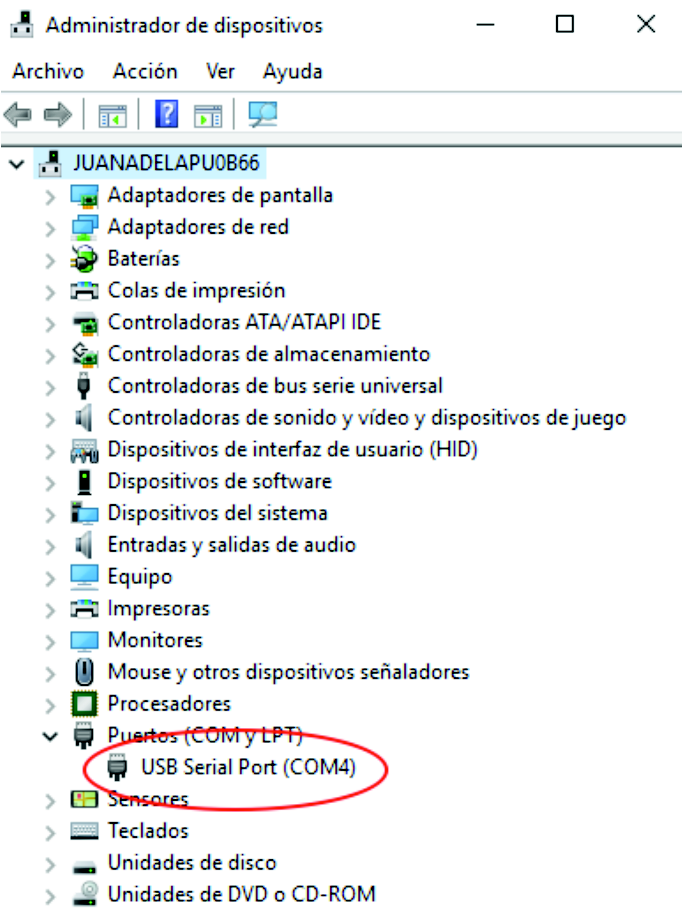
\includegraphics[width=0.6\textwidth,keepaspectratio]{com.png}}
            \caption{Identification of usb serial port.}
            \label{fig:com}
\end{figure}

Now, to set up PuTTY, open the application and set the configuration parameters as shown in figure~\ref{fig:cable}.

\begin{figure}[h]
            \centering{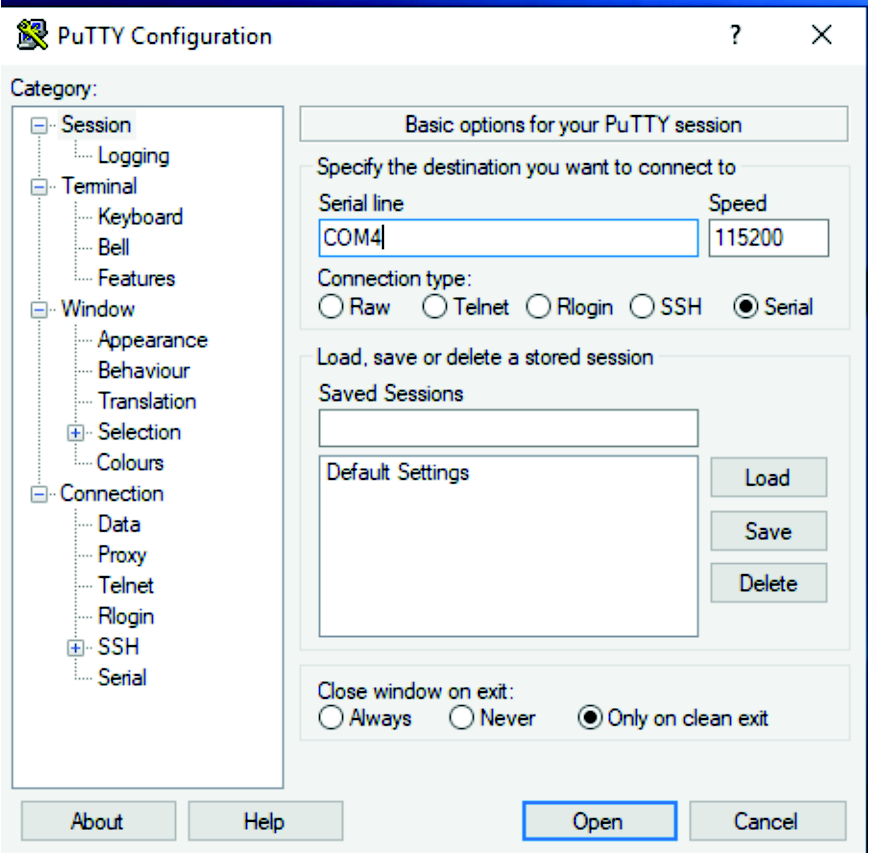
\includegraphics[width=0.6\textwidth,keepaspectratio]{putty.png}}
            \caption{PuTTY configuration.}
            \label{fig:putty}
\end{figure}

\subsection{MacOS}
The recommended application is screen, which is already installed in MacOS.
First you have to identify the USB serial port. Open a terminal window and type
\begin{verbatim}
\$ ls /dev | grep -i usb
\end{verbatim}
You will get a list of devices like the following:
\begin{verbatim}
cu.usbserial-FTA5I24G
tty.usbserial-FTA5I24G
\end{verbatim}

As you can see, there are two devices for each serial line. You can use any of them, but for reasons not to be discussed here it is better, in general, to use the one starting with cu.

To use the screen application enter the following command:
\begin{verbatim}
\$ screen /dev/cu.usbserial-XXXX 115200
\end{verbatim}

where {\tt /dev/cu.usbserial-XXXX} is the name of your device.

To exit the application, type CTRL-A and then CTRL-K.

\subsection{GNU Linux}

The recommended application is screen\footnote{{\tt gtkterm} or {\tt kermit} are good alternatives}, which can be installed in Ubuntu Linux with:
\begin{verbatim}
\$ sudo apt install screen
\end{verbatim}

In order to identify the USB serial port, type the following command on a terminal:

\begin{verbatim}
\$ ls /dev | grep -i usb
\end{verbatim}

You will get a result like the following:
\begin{verbatim}
ttyUSB0
\end{verbatim}

To use the screen application enter the following command:

\begin{verbatim}
\$ screen /dev/ttyUSB0 115200
\end{verbatim}

To exit the application, type CTRL-A and then SHIFT-K.

\section{Software architecture}

The software architecture is similar to the previous project, except that the display is replaced by a serial line handler adapted from the examples in the Ada Drivers Library.


\begin{figure}[h]
            \centering{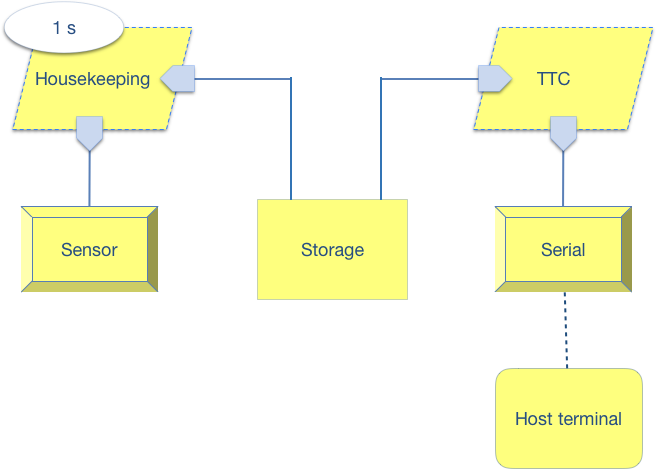
\includegraphics[width=0.6\textwidth,keepaspectratio]{distributed.png}}
            \caption{Software architecture of distributed housekeeping system.}
            \label{fig:distributed}
\end{figure}

\subsection{Download the code and study the implementation}

The implementation code, as initially provided to the students, can be downloaded from \url{https://github.com/STR-UPM/OBDH_LABS}. Click on {\tt Clone} or {\tt download}, download a zip archive, unzip and move to your work directory. The code for this assignment is in the LAB5 folder.

The {\tt Serial} component is implemented by the {\tt Serial.IO} package and other packages in the {\tt serial\_ports} folder. These packages have been adapted from the examples in the Ada Drivers Library. The blocking kind of serial port has been chosen for this project. This means that the task calling the {\tt Put} operation ({\tt TM\_Task}) waits on a busy loop until the operation is complete.

The rest of the implementation is the same as in the previous project.

\section{Compile and run.}

Open GPS and do the following:
\begin{enumerate}
\item Select {\tt Open} project on the welcome window. Navigate to the LAB5 directory and open the {\tt distributed\_housekeeping.gpr} project file.
\item Build the executable and load it into the board by clicking on the \hbox{
\includegraphics[width=1.5em]{buildandload.png}} symbol in the tool bar (or select {\tt Build} > {\tt Bareboard} > {\tt Flash to board} on the top menu).

The program will be compiled, and the executable will be loaded into the board flash memory. After that, the program starts to run on the board (check the blinking LEDs).
\item Connect the serial cable to a USB port on the host computer, if not already done.
\item Identify the serial port name on the host computer and launch the remote terminal application as explained in section~\ref{sc:term}. The sensor measured values will start being displayed on the host application.
\end{enumerate}


\section{Make changes to the program}

You may include the same changes that were proposed in the previous assignment:

\begin{enumerate}
\item Include the conversion to Celsius in the {\tt Display.Put} procedure.
\end{enumerate}
